% Options for packages loaded elsewhere
\PassOptionsToPackage{unicode}{hyperref}
\PassOptionsToPackage{hyphens}{url}
%
\documentclass[
]{book}
\usepackage{amsmath,amssymb}
\usepackage{lmodern}
\usepackage{iftex}
\ifPDFTeX
  \usepackage[T1]{fontenc}
  \usepackage[utf8]{inputenc}
  \usepackage{textcomp} % provide euro and other symbols
\else % if luatex or xetex
  \usepackage{unicode-math}
  \defaultfontfeatures{Scale=MatchLowercase}
  \defaultfontfeatures[\rmfamily]{Ligatures=TeX,Scale=1}
\fi
% Use upquote if available, for straight quotes in verbatim environments
\IfFileExists{upquote.sty}{\usepackage{upquote}}{}
\IfFileExists{microtype.sty}{% use microtype if available
  \usepackage[]{microtype}
  \UseMicrotypeSet[protrusion]{basicmath} % disable protrusion for tt fonts
}{}
\makeatletter
\@ifundefined{KOMAClassName}{% if non-KOMA class
  \IfFileExists{parskip.sty}{%
    \usepackage{parskip}
  }{% else
    \setlength{\parindent}{0pt}
    \setlength{\parskip}{6pt plus 2pt minus 1pt}}
}{% if KOMA class
  \KOMAoptions{parskip=half}}
\makeatother
\usepackage{xcolor}
\IfFileExists{xurl.sty}{\usepackage{xurl}}{} % add URL line breaks if available
\IfFileExists{bookmark.sty}{\usepackage{bookmark}}{\usepackage{hyperref}}
\hypersetup{
  pdftitle={797ML Handbook},
  pdfauthor={Steve Linberg},
  hidelinks,
  pdfcreator={LaTeX via pandoc}}
\urlstyle{same} % disable monospaced font for URLs
\usepackage{color}
\usepackage{fancyvrb}
\newcommand{\VerbBar}{|}
\newcommand{\VERB}{\Verb[commandchars=\\\{\}]}
\DefineVerbatimEnvironment{Highlighting}{Verbatim}{commandchars=\\\{\}}
% Add ',fontsize=\small' for more characters per line
\usepackage{framed}
\definecolor{shadecolor}{RGB}{248,248,248}
\newenvironment{Shaded}{\begin{snugshade}}{\end{snugshade}}
\newcommand{\AlertTok}[1]{\textcolor[rgb]{0.94,0.16,0.16}{#1}}
\newcommand{\AnnotationTok}[1]{\textcolor[rgb]{0.56,0.35,0.01}{\textbf{\textit{#1}}}}
\newcommand{\AttributeTok}[1]{\textcolor[rgb]{0.77,0.63,0.00}{#1}}
\newcommand{\BaseNTok}[1]{\textcolor[rgb]{0.00,0.00,0.81}{#1}}
\newcommand{\BuiltInTok}[1]{#1}
\newcommand{\CharTok}[1]{\textcolor[rgb]{0.31,0.60,0.02}{#1}}
\newcommand{\CommentTok}[1]{\textcolor[rgb]{0.56,0.35,0.01}{\textit{#1}}}
\newcommand{\CommentVarTok}[1]{\textcolor[rgb]{0.56,0.35,0.01}{\textbf{\textit{#1}}}}
\newcommand{\ConstantTok}[1]{\textcolor[rgb]{0.00,0.00,0.00}{#1}}
\newcommand{\ControlFlowTok}[1]{\textcolor[rgb]{0.13,0.29,0.53}{\textbf{#1}}}
\newcommand{\DataTypeTok}[1]{\textcolor[rgb]{0.13,0.29,0.53}{#1}}
\newcommand{\DecValTok}[1]{\textcolor[rgb]{0.00,0.00,0.81}{#1}}
\newcommand{\DocumentationTok}[1]{\textcolor[rgb]{0.56,0.35,0.01}{\textbf{\textit{#1}}}}
\newcommand{\ErrorTok}[1]{\textcolor[rgb]{0.64,0.00,0.00}{\textbf{#1}}}
\newcommand{\ExtensionTok}[1]{#1}
\newcommand{\FloatTok}[1]{\textcolor[rgb]{0.00,0.00,0.81}{#1}}
\newcommand{\FunctionTok}[1]{\textcolor[rgb]{0.00,0.00,0.00}{#1}}
\newcommand{\ImportTok}[1]{#1}
\newcommand{\InformationTok}[1]{\textcolor[rgb]{0.56,0.35,0.01}{\textbf{\textit{#1}}}}
\newcommand{\KeywordTok}[1]{\textcolor[rgb]{0.13,0.29,0.53}{\textbf{#1}}}
\newcommand{\NormalTok}[1]{#1}
\newcommand{\OperatorTok}[1]{\textcolor[rgb]{0.81,0.36,0.00}{\textbf{#1}}}
\newcommand{\OtherTok}[1]{\textcolor[rgb]{0.56,0.35,0.01}{#1}}
\newcommand{\PreprocessorTok}[1]{\textcolor[rgb]{0.56,0.35,0.01}{\textit{#1}}}
\newcommand{\RegionMarkerTok}[1]{#1}
\newcommand{\SpecialCharTok}[1]{\textcolor[rgb]{0.00,0.00,0.00}{#1}}
\newcommand{\SpecialStringTok}[1]{\textcolor[rgb]{0.31,0.60,0.02}{#1}}
\newcommand{\StringTok}[1]{\textcolor[rgb]{0.31,0.60,0.02}{#1}}
\newcommand{\VariableTok}[1]{\textcolor[rgb]{0.00,0.00,0.00}{#1}}
\newcommand{\VerbatimStringTok}[1]{\textcolor[rgb]{0.31,0.60,0.02}{#1}}
\newcommand{\WarningTok}[1]{\textcolor[rgb]{0.56,0.35,0.01}{\textbf{\textit{#1}}}}
\usepackage{longtable,booktabs,array}
\usepackage{calc} % for calculating minipage widths
% Correct order of tables after \paragraph or \subparagraph
\usepackage{etoolbox}
\makeatletter
\patchcmd\longtable{\par}{\if@noskipsec\mbox{}\fi\par}{}{}
\makeatother
% Allow footnotes in longtable head/foot
\IfFileExists{footnotehyper.sty}{\usepackage{footnotehyper}}{\usepackage{footnote}}
\makesavenoteenv{longtable}
\usepackage{graphicx}
\makeatletter
\def\maxwidth{\ifdim\Gin@nat@width>\linewidth\linewidth\else\Gin@nat@width\fi}
\def\maxheight{\ifdim\Gin@nat@height>\textheight\textheight\else\Gin@nat@height\fi}
\makeatother
% Scale images if necessary, so that they will not overflow the page
% margins by default, and it is still possible to overwrite the defaults
% using explicit options in \includegraphics[width, height, ...]{}
\setkeys{Gin}{width=\maxwidth,height=\maxheight,keepaspectratio}
% Set default figure placement to htbp
\makeatletter
\def\fps@figure{htbp}
\makeatother
\setlength{\emergencystretch}{3em} % prevent overfull lines
\providecommand{\tightlist}{%
  \setlength{\itemsep}{0pt}\setlength{\parskip}{0pt}}
\setcounter{secnumdepth}{5}
\usepackage{booktabs}
\ifLuaTeX
  \usepackage{selnolig}  % disable illegal ligatures
\fi
\usepackage[]{natbib}
\bibliographystyle{plainnat}

\title{797ML Handbook}
\author{Steve Linberg}
\date{2022-04-03}

\begin{document}
\maketitle

{
\setcounter{tocdepth}{1}
\tableofcontents
}
\hypertarget{about}{%
\chapter{About}\label{about}}

This book is being written as part of a final project for 797ML at UMass
Amherst, spring 2022. It contains a simple reference and breakdown for a
couple of dozen core methods used in machine learning.

The intent is twofold:

\begin{enumerate}
\def\labelenumi{\arabic{enumi}.}
\tightlist
\item
  Serve as a reference for the basics of the material covered in the class, using language and examples that are as simple as possible to explain the core concepts and how to do them;
\item
  Force myself to learn these techniques better by carrying out the above.
\end{enumerate}

The main purpose of this work is to be \emph{simple}, not to be \emph{comprehensive}. We won't cover every facet of every technique, or every possible permutations of outcomes. The goal is to simply express the broad strokes and core concepts in a way that can be easily remembered, and to serve as a jumping-off point when more information is needed.

\hypertarget{authoring-guidelines}{%
\section{Authoring guidelines}\label{authoring-guidelines}}

The goal is to have no more than a few short paragraphs for each section, and to keep each explanation of the meanings of outcome variables to one sentence each.

\hypertarget{resources}{%
\section{Resources}\label{resources}}

A lot of the material from this work is from the class textbook, \citet{ISLR}. I also find UNC geneticist Josh Starmer's \href{https://www.youtube.com/channel/UCtYLUTtgS3k1Fg4y5tAhLbw}{StatQuest} video series on YouTube to be immensely helpful for simple explanations of statistics and machine learning concepts.

\hypertarget{simple-linear-regression}{%
\chapter{Simple Linear Regression}\label{simple-linear-regression}}

\hypertarget{tldr}{%
\section{TL;DR}\label{tldr}}

\begin{description}
\tightlist
\item[What it does]
Looks to see how well a single predictor variable predicts an outcome, like \emph{how well do years of education predict salary?}
\item[When to do it]
When you want to see if pretty much the simplest possible model provides enough of an explanation of variance for your purposes
\item[How to do it]
With the \texttt{lm()} function, among other ways
\item[How to assess it]
Look for a significant \(p\)-value for the predictor, and a reasonable \(R^2\)
\end{description}

\hypertarget{what-it-does}{%
\section{What it does}\label{what-it-does}}

Simple linear regression is where it all begins; among the simplest of all of the regression techniques in analysis, which attempts to estimate a slope and an intercept line for a set of observations using a single predictor variable \(X\) and an output variable \(Y\). It uses ordinary least squares (OLS) to build its model, looking for the line through the mean of \(X\) and \(Y\) that has the smallest sum of squares between the predicted and observed values.



\begin{figure}
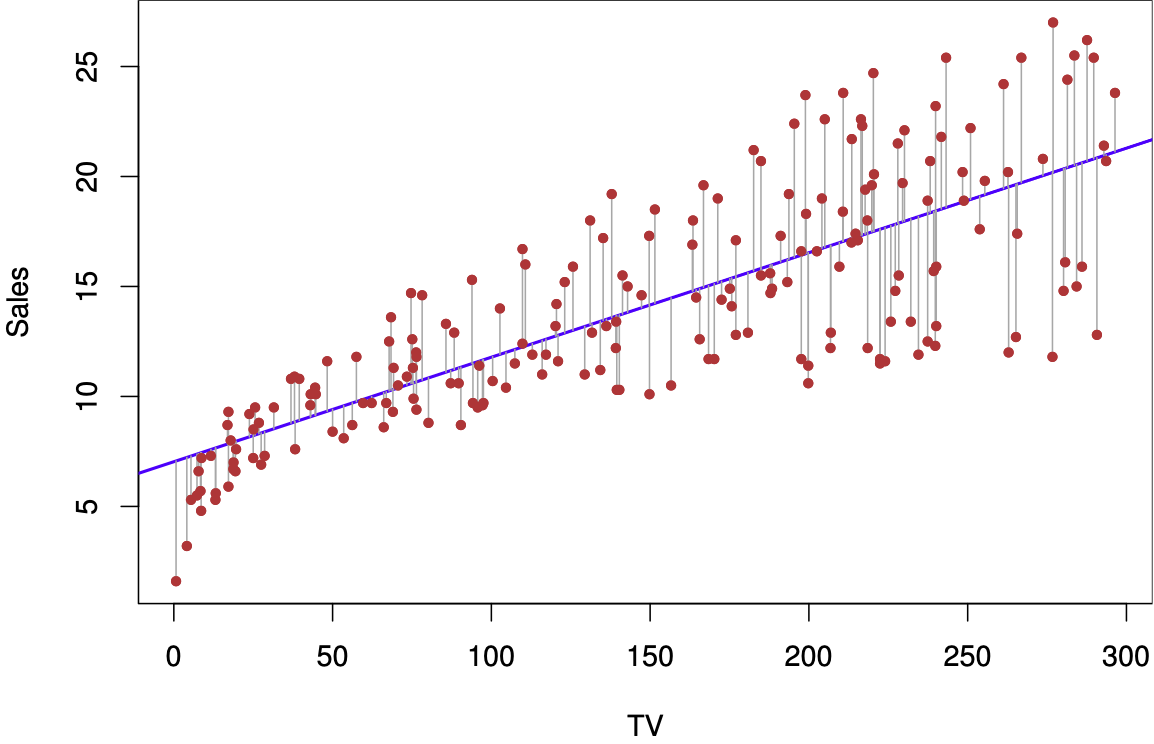
\includegraphics[width=16.03in]{images/3_1} \caption{Simple linear regression plot (source: \citet{ISLR}, p.~62)}\label{fig:img-slr1}
\end{figure}

The figure above shows a plot of a simple linear regression, attempting to use the variable \texttt{TV} to predict \texttt{Sales.} The blue line is the line defined by the regression with its \(Y\) intercept and slope; the red dots are the actual observations of \texttt{Sales} for each measure of the predictor \texttt{TV} on the \(X\) axis. The thin blue lines are the error in the prediction.

\hypertarget{when-to-do-it}{%
\section{When to do it}\label{when-to-do-it}}

It is a simple first step for looking at data to see if there is an easy single-variable model that does a reasonable job predicting outcomes using one predictor variable. Sometimes, it can be good enough! It has the advantage of being easy to execute, to understand and to communicate, and the value of these factors should not be underestimated. Communicating with non-specialists is an important aspect of a data scientist's job.

Linear regression requires a dataset with a continuous outcome variable; it is easiest and most effective if the predictor variable is also numeric, whether continuous or discrete. It is possible to do linear regression with non-numeric predictors, such as true/false or ordered responses, by converting the predictors to a numeric scale.

\hypertarget{how-to-do-it}{%
\section{How to do it}\label{how-to-do-it}}

This example from \citet{ISLR} shows a simple linear regression of \textbf{medv} onto \textbf{lstat}, attempting to predict median housing prices from percentage of ``lower-status'' population in the Boston data set from the late 1970s.

\begin{Shaded}
\begin{Highlighting}[]
\NormalTok{lm.fit }\OtherTok{\textless{}{-}} \FunctionTok{lm}\NormalTok{(medv }\SpecialCharTok{\textasciitilde{}}\NormalTok{ lstat, }\AttributeTok{data =}\NormalTok{ Boston)}
\FunctionTok{plot}\NormalTok{(Boston}\SpecialCharTok{$}\NormalTok{lstat, Boston}\SpecialCharTok{$}\NormalTok{medv)}
\FunctionTok{abline}\NormalTok{(lm.fit, }\AttributeTok{lwd =} \DecValTok{3}\NormalTok{, }\AttributeTok{col =} \StringTok{"red"}\NormalTok{)}
\end{Highlighting}
\end{Shaded}

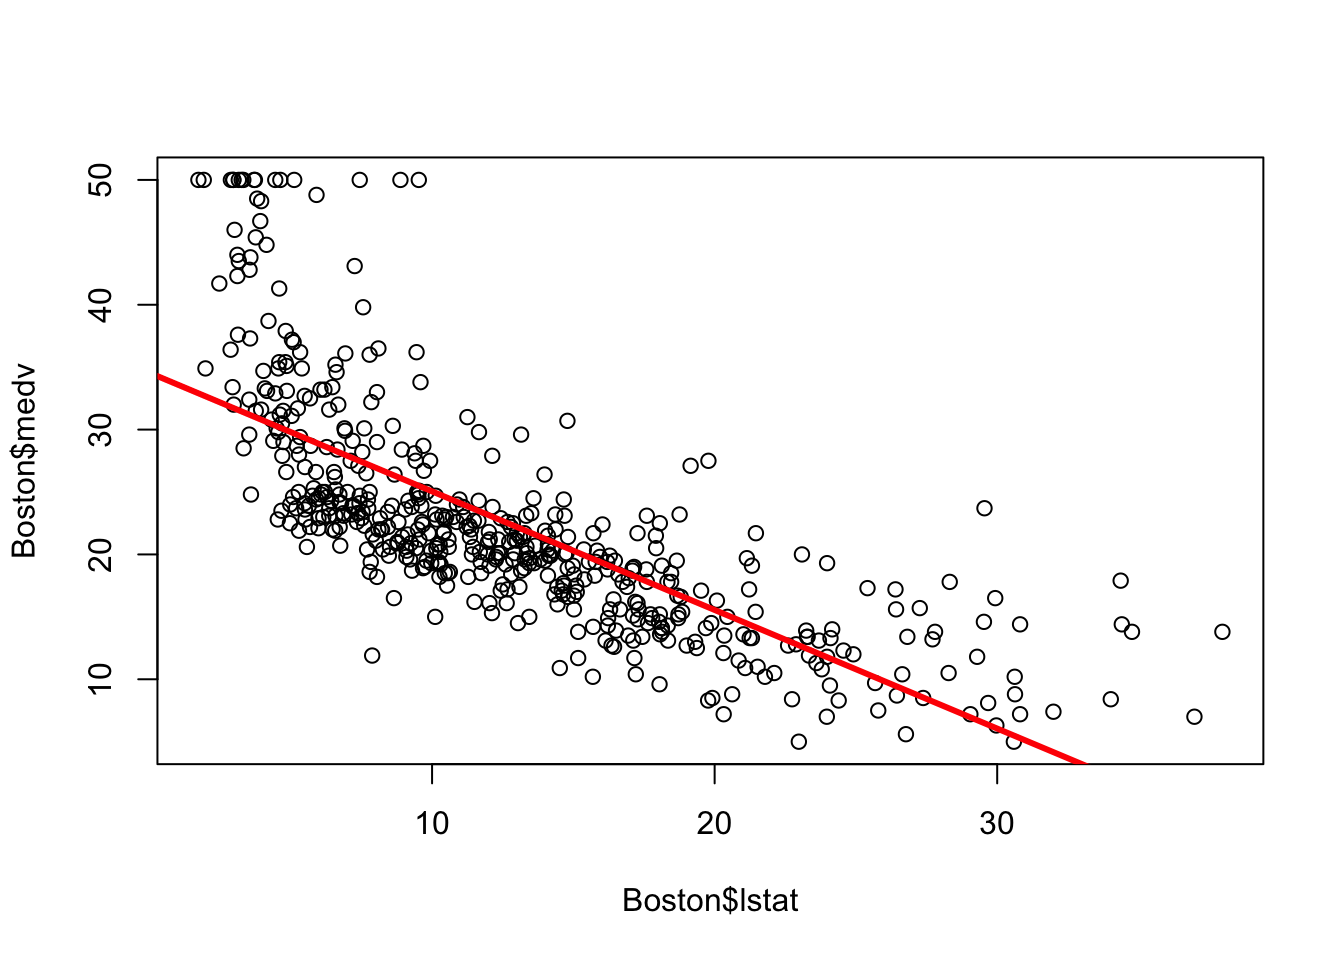
\includegraphics{_main_files/figure-latex/unnamed-chunk-3-1.pdf}

The results of the regression are stored in the output of \texttt{lm()}, and may be viewed with \texttt{summary()}:

\begin{Shaded}
\begin{Highlighting}[]
\FunctionTok{summary}\NormalTok{(lm.fit)}
\end{Highlighting}
\end{Shaded}

\begin{verbatim}
## 
## Call:
## lm(formula = medv ~ lstat, data = Boston)
## 
## Residuals:
##     Min      1Q  Median      3Q     Max 
## -15.168  -3.990  -1.318   2.034  24.500 
## 
## Coefficients:
##             Estimate Std. Error t value Pr(>|t|)    
## (Intercept) 34.55384    0.56263   61.41   <2e-16 ***
## lstat       -0.95005    0.03873  -24.53   <2e-16 ***
## ---
## Signif. codes:  0 '***' 0.001 '**' 0.01 '*' 0.05 '.' 0.1 ' ' 1
## 
## Residual standard error: 6.216 on 504 degrees of freedom
## Multiple R-squared:  0.5441, Adjusted R-squared:  0.5432 
## F-statistic: 601.6 on 1 and 504 DF,  p-value: < 2.2e-16
\end{verbatim}

\hypertarget{how-to-interpret-the-output}{%
\section{How to interpret the output}\label{how-to-interpret-the-output}}

The output contains a lot of information, but the key points are:

\begin{itemize}
\tightlist
\item
  \texttt{Adjusted\ R-squared}: 0.5432 is the percentage of the variation in the model that is explained by the fit's prediction, compared to just looking at how much the observations vary from their own average with no predictor variable.
\item
  \texttt{p-value}: \textless{} 2.2e-16 (basically zero) means that the model is (very) statistically significant, with a near-zero percent chance that the data in this set could have resulted from a random draw from the (unknown) population if there were no relationship between \texttt{medv} and \texttt{lstat}
\item
  \texttt{Estimated\ intercept} of 34.55 is the \(Y\) intercept on the graph, or the estimated value of \texttt{medv} when \texttt{lstat} is zero
\item
  \texttt{Estimated\ (lstat)}: -0.95 is the estimated coefficient of \texttt{lstat}, or the amount that \texttt{medv} changes by for each unit change in \texttt{lstat}.
\end{itemize}

The intercept and coefficient are \(\beta_0\) and \(\beta_1\), respectively, of the linear regression formula

\[Y = \beta_0 + \beta_1X\]
Substituting the coefficients and variables, we transform this to:

\[\text{medv} = 34.55 - 0.95 \times \text{lstat}\]

The low p-value shows that there is (almost) definitely a relationship between \texttt{medv} and \texttt{lstat}, but the \(R^2\) of 0.54 shows that the model only explains slightly more than half of the variation in the data. It's not a bad start, but we would probably want to find a model that explains more of it.

\hypertarget{where-to-learn-more}{%
\section{Where to learn more}\label{where-to-learn-more}}

\begin{itemize}
\tightlist
\item
  Chapter 3 - 3.1 in \citet{ISLR}
\item
  \href{https://www.youtube.com/watch?v=nk2CQITm_eo}{StatQuest: Linear Regression} - this goes into good depth on the meaning of the \(F\) statistic as well, and how it used to calculate the \(p\) value.
\end{itemize}

\hypertarget{notes}{%
\section{Notes}\label{notes}}

You can also do a scatterplot in ggplot2 and add a regression line with \texttt{geom\_smooth()}; it doesn't show the coefficients or other output information, but it gives a quick visual that's a little prettier than the base R plot:

\begin{Shaded}
\begin{Highlighting}[]
\FunctionTok{ggplot}\NormalTok{(}\AttributeTok{data =}\NormalTok{ Boston, }\FunctionTok{aes}\NormalTok{(}\AttributeTok{x =}\NormalTok{ lstat, }\AttributeTok{y =}\NormalTok{ medv)) }\SpecialCharTok{+}
  \FunctionTok{geom\_point}\NormalTok{(}\AttributeTok{alpha =} \FloatTok{0.5}\NormalTok{) }\SpecialCharTok{+}
  \FunctionTok{geom\_smooth}\NormalTok{(}\AttributeTok{method =} \StringTok{"lm"}\NormalTok{, }\AttributeTok{formula =}\NormalTok{ y }\SpecialCharTok{\textasciitilde{}}\NormalTok{ x) }\SpecialCharTok{+}
  \FunctionTok{geom\_hline}\NormalTok{(}\AttributeTok{yintercept =} \FunctionTok{mean}\NormalTok{(Boston}\SpecialCharTok{$}\NormalTok{medv), }\AttributeTok{linetype =} \StringTok{"dashed"}\NormalTok{, }\AttributeTok{color =} \StringTok{"red"}\NormalTok{) }\SpecialCharTok{+}
  \FunctionTok{geom\_vline}\NormalTok{(}\AttributeTok{xintercept =} \FunctionTok{mean}\NormalTok{(Boston}\SpecialCharTok{$}\NormalTok{lstat), }\AttributeTok{linetype =} \StringTok{"dashed"}\NormalTok{, }\AttributeTok{color =} \StringTok{"darkgreen"}\NormalTok{) }\SpecialCharTok{+}
  \FunctionTok{theme\_minimal}\NormalTok{()}
\end{Highlighting}
\end{Shaded}

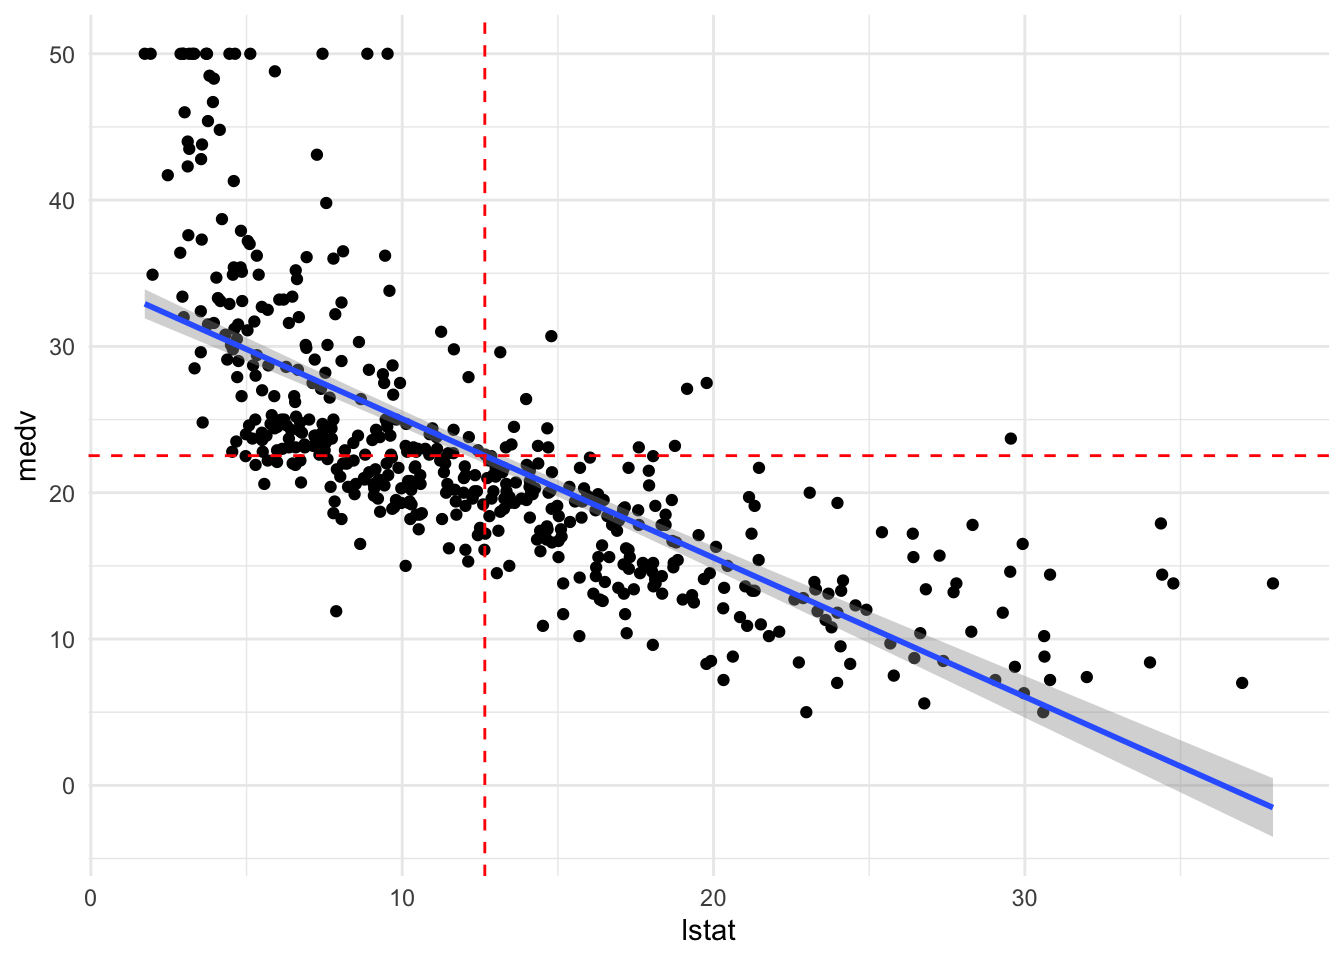
\includegraphics{_main_files/figure-latex/unnamed-chunk-5-1.pdf}

The means of \texttt{lstat} and \texttt{medv} are shown with dashed red and green lines, showing that the regression line goes through the center of the data.

\hypertarget{multiple-linear-regression}{%
\chapter{Multiple Linear Regression}\label{multiple-linear-regression}}

\hypertarget{tldr-1}{%
\section{TL;DR}\label{tldr-1}}

\begin{description}
\tightlist
\item[What it does]
Looks to see how well multiple predictor variables predict an outcome, like \emph{how well do years of education and age predict salary?}
\item[When to do it]
When a \protect\hyperlink{simple-linear-regression}{simple linear regression} doesn't provide a good enough explanation of variance, and you want to see if adding additional variables provides a better one
\item[How to do it]
With the \texttt{lm()} function, utilizing more than one predictor
\item[How to assess it]
Look for significant \(p\)-values for the predictors, and a reasonable adjusted-\(R^2\)
\end{description}

\hypertarget{what-it-does-1}{%
\section{What it does}\label{what-it-does-1}}

Multiple linear regression is the first natural extension of simple linear regression. It allows for more than one predictor variable to be specified. It is also possible to combine predictors in interactions, to find out if combinations of predictors have different effects than simply adding them to the model. XXX explain/demo

\hypertarget{when-to-do-it-1}{%
\section{When to do it}\label{when-to-do-it-1}}

Use multiple linear regression when a simple linear regression doesn't provide a good enough explanation of the variance you're observing, and you want to see if adding more predictors provides a better fit. Typically, this would be in response to either a low \(R^2\) that leaves a lot of unexplained variance, or even just a visual conclusion drawn from seeing a plot of a linear model with an unsatisfactory regression line.

\hypertarget{how-to-do-it-1}{%
\section{How to do it}\label{how-to-do-it-1}}

The \texttt{lm()} function, using more than one predictor in the formula.

\hypertarget{how-to-interpret-the-output-1}{%
\section{How to interpret the output}\label{how-to-interpret-the-output-1}}

\hypertarget{where-to-learn-more-1}{%
\section{Where to learn more}\label{where-to-learn-more-1}}

\hypertarget{logistic-regression}{%
\chapter{Logistic Regression}\label{logistic-regression}}

\hypertarget{tldr-2}{%
\section{TL;DR}\label{tldr-2}}

What it does
:

When to do it
:

How to do it
:

How to assess it
:

\hypertarget{what-it-does-2}{%
\section{What it does}\label{what-it-does-2}}

\hypertarget{when-to-do-it-2}{%
\section{When to do it}\label{when-to-do-it-2}}

\hypertarget{how-to-do-it-2}{%
\section{How to do it}\label{how-to-do-it-2}}

\hypertarget{how-to-interpret-the-output-2}{%
\section{How to interpret the output}\label{how-to-interpret-the-output-2}}

\hypertarget{where-to-learn-more-2}{%
\section{Where to learn more}\label{where-to-learn-more-2}}

\hypertarget{multiple-logistic-regression}{%
\chapter{Multiple Logistic Regression}\label{multiple-logistic-regression}}

\hypertarget{tldr-3}{%
\section{TL;DR}\label{tldr-3}}

What it does
:

When to do it
:

How to do it
:

How to assess it
:

\hypertarget{what-it-does-3}{%
\section{What it does}\label{what-it-does-3}}

\hypertarget{when-to-do-it-3}{%
\section{When to do it}\label{when-to-do-it-3}}

\hypertarget{how-to-do-it-3}{%
\section{How to do it}\label{how-to-do-it-3}}

\hypertarget{how-to-interpret-the-output-3}{%
\section{How to interpret the output}\label{how-to-interpret-the-output-3}}

\hypertarget{where-to-learn-more-3}{%
\section{Where to learn more}\label{where-to-learn-more-3}}

\hypertarget{linear-discriminant-analysis}{%
\chapter{Linear Discriminant Analysis}\label{linear-discriminant-analysis}}

\hypertarget{tldr-4}{%
\section{TL;DR}\label{tldr-4}}

What it does
:

When to do it
:

How to do it
:

How to assess it
:

\hypertarget{what-it-does-4}{%
\section{What it does}\label{what-it-does-4}}

\hypertarget{when-to-do-it-4}{%
\section{When to do it}\label{when-to-do-it-4}}

\hypertarget{how-to-do-it-4}{%
\section{How to do it}\label{how-to-do-it-4}}

\hypertarget{how-to-interpret-the-output-4}{%
\section{How to interpret the output}\label{how-to-interpret-the-output-4}}

\hypertarget{where-to-learn-more-4}{%
\section{Where to learn more}\label{where-to-learn-more-4}}

\hypertarget{quadratic-discriminant-analysis}{%
\chapter{Quadratic Discriminant Analysis}\label{quadratic-discriminant-analysis}}

\hypertarget{tldr-5}{%
\section{TL;DR}\label{tldr-5}}

What it does
:

When to do it
:

How to do it
:

How to assess it
:

\hypertarget{what-it-does-5}{%
\section{What it does}\label{what-it-does-5}}

\hypertarget{when-to-do-it-5}{%
\section{When to do it}\label{when-to-do-it-5}}

\hypertarget{how-to-do-it-5}{%
\section{How to do it}\label{how-to-do-it-5}}

\hypertarget{how-to-interpret-the-output-5}{%
\section{How to interpret the output}\label{how-to-interpret-the-output-5}}

\hypertarget{where-to-learn-more-5}{%
\section{Where to learn more}\label{where-to-learn-more-5}}

\hypertarget{naive-bayes}{%
\chapter{Naive Bayes}\label{naive-bayes}}

\hypertarget{tldr-6}{%
\section{TL;DR}\label{tldr-6}}

What it does
:

When to do it
:

How to do it
:

How to assess it
:

\hypertarget{what-it-does-6}{%
\section{What it does}\label{what-it-does-6}}

\hypertarget{when-to-do-it-6}{%
\section{When to do it}\label{when-to-do-it-6}}

\hypertarget{how-to-do-it-6}{%
\section{How to do it}\label{how-to-do-it-6}}

\hypertarget{how-to-interpret-the-output-6}{%
\section{How to interpret the output}\label{how-to-interpret-the-output-6}}

\hypertarget{where-to-learn-more-6}{%
\section{Where to learn more}\label{where-to-learn-more-6}}

\hypertarget{k-nearest-neighbors}{%
\chapter{K-Nearest Neighbors}\label{k-nearest-neighbors}}

\hypertarget{tldr-7}{%
\section{TL;DR}\label{tldr-7}}

What it does
:

When to do it
:

How to do it
:

How to assess it
:

\hypertarget{what-it-does-7}{%
\section{What it does}\label{what-it-does-7}}

\hypertarget{when-to-do-it-7}{%
\section{When to do it}\label{when-to-do-it-7}}

\hypertarget{how-to-do-it-7}{%
\section{How to do it}\label{how-to-do-it-7}}

\hypertarget{how-to-interpret-the-output-7}{%
\section{How to interpret the output}\label{how-to-interpret-the-output-7}}

\hypertarget{where-to-learn-more-7}{%
\section{Where to learn more}\label{where-to-learn-more-7}}

\hypertarget{poisson-regression}{%
\chapter{Poisson Regression}\label{poisson-regression}}

\hypertarget{tldr-8}{%
\section{TL;DR}\label{tldr-8}}

What it does
:

When to do it
:

How to do it
:

How to assess it
:

\hypertarget{what-it-does-8}{%
\section{What it does}\label{what-it-does-8}}

\hypertarget{when-to-do-it-8}{%
\section{When to do it}\label{when-to-do-it-8}}

\hypertarget{how-to-do-it-8}{%
\section{How to do it}\label{how-to-do-it-8}}

\hypertarget{how-to-interpret-the-output-8}{%
\section{How to interpret the output}\label{how-to-interpret-the-output-8}}

\hypertarget{where-to-learn-more-8}{%
\section{Where to learn more}\label{where-to-learn-more-8}}

\hypertarget{cross-validation}{%
\chapter{Cross-Validation}\label{cross-validation}}

\hypertarget{tldr-9}{%
\section{TL;DR}\label{tldr-9}}

What it does
:

When to do it
:

How to do it
:

How to assess it
:

\hypertarget{what-it-does-9}{%
\section{What it does}\label{what-it-does-9}}

\hypertarget{when-to-do-it-9}{%
\section{When to do it}\label{when-to-do-it-9}}

\hypertarget{how-to-do-it-9}{%
\section{How to do it}\label{how-to-do-it-9}}

\hypertarget{how-to-interpret-the-output-9}{%
\section{How to interpret the output}\label{how-to-interpret-the-output-9}}

\hypertarget{where-to-learn-more-9}{%
\section{Where to learn more}\label{where-to-learn-more-9}}

\hypertarget{bootstrap}{%
\chapter{Bootstrap}\label{bootstrap}}

\hypertarget{tldr-10}{%
\section{TL;DR}\label{tldr-10}}

What it does
:

When to do it
:

How to do it
:

How to assess it
:

\hypertarget{what-it-does-10}{%
\section{What it does}\label{what-it-does-10}}

\hypertarget{when-to-do-it-10}{%
\section{When to do it}\label{when-to-do-it-10}}

\hypertarget{how-to-do-it-10}{%
\section{How to do it}\label{how-to-do-it-10}}

\hypertarget{how-to-interpret-the-output-10}{%
\section{How to interpret the output}\label{how-to-interpret-the-output-10}}

\hypertarget{where-to-learn-more-10}{%
\section{Where to learn more}\label{where-to-learn-more-10}}

\hypertarget{best-subset-selection}{%
\chapter{Best Subset Selection}\label{best-subset-selection}}

\hypertarget{tldr-11}{%
\section{TL;DR}\label{tldr-11}}

What it does
:

When to do it
:

How to do it
:

How to assess it
:

\hypertarget{what-it-does-11}{%
\section{What it does}\label{what-it-does-11}}

\hypertarget{when-to-do-it-11}{%
\section{When to do it}\label{when-to-do-it-11}}

\hypertarget{how-to-do-it-11}{%
\section{How to do it}\label{how-to-do-it-11}}

\hypertarget{how-to-interpret-the-output-11}{%
\section{How to interpret the output}\label{how-to-interpret-the-output-11}}

\hypertarget{where-to-learn-more-11}{%
\section{Where to learn more}\label{where-to-learn-more-11}}

\hypertarget{stepwise-selection}{%
\chapter{Stepwise Selection}\label{stepwise-selection}}

\hypertarget{tldr-12}{%
\section{TL;DR}\label{tldr-12}}

What it does
:

When to do it
:

How to do it
:

How to assess it
:

\hypertarget{what-it-does-12}{%
\section{What it does}\label{what-it-does-12}}

\hypertarget{when-to-do-it-12}{%
\section{When to do it}\label{when-to-do-it-12}}

\hypertarget{how-to-do-it-12}{%
\section{How to do it}\label{how-to-do-it-12}}

\hypertarget{how-to-interpret-the-output-12}{%
\section{How to interpret the output}\label{how-to-interpret-the-output-12}}

\hypertarget{where-to-learn-more-12}{%
\section{Where to learn more}\label{where-to-learn-more-12}}

\hypertarget{ridge-regression}{%
\chapter{Ridge Regression}\label{ridge-regression}}

\hypertarget{tldr-13}{%
\section{TL;DR}\label{tldr-13}}

What it does
:

When to do it
:

How to do it
:

How to assess it
:

\hypertarget{what-it-does-13}{%
\section{What it does}\label{what-it-does-13}}

\hypertarget{when-to-do-it-13}{%
\section{When to do it}\label{when-to-do-it-13}}

\hypertarget{how-to-do-it-13}{%
\section{How to do it}\label{how-to-do-it-13}}

\hypertarget{how-to-interpret-the-output-13}{%
\section{How to interpret the output}\label{how-to-interpret-the-output-13}}

\hypertarget{where-to-learn-more-13}{%
\section{Where to learn more}\label{where-to-learn-more-13}}

\hypertarget{lasso}{%
\chapter{Lasso}\label{lasso}}

\hypertarget{tldr-14}{%
\section{TL;DR}\label{tldr-14}}

What it does
:

When to do it
:

How to do it
:

How to assess it
:

\hypertarget{what-it-does-14}{%
\section{What it does}\label{what-it-does-14}}

\hypertarget{when-to-do-it-14}{%
\section{When to do it}\label{when-to-do-it-14}}

\hypertarget{how-to-do-it-14}{%
\section{How to do it}\label{how-to-do-it-14}}

\hypertarget{how-to-interpret-the-output-14}{%
\section{How to interpret the output}\label{how-to-interpret-the-output-14}}

\hypertarget{where-to-learn-more-14}{%
\section{Where to learn more}\label{where-to-learn-more-14}}

\hypertarget{principal-component-regression}{%
\chapter{Principal Component Regression}\label{principal-component-regression}}

\hypertarget{tldr-15}{%
\section{TL;DR}\label{tldr-15}}

What it does
:

When to do it
:

How to do it
:

How to assess it
:

\hypertarget{what-it-does-15}{%
\section{What it does}\label{what-it-does-15}}

\hypertarget{when-to-do-it-15}{%
\section{When to do it}\label{when-to-do-it-15}}

\hypertarget{how-to-do-it-15}{%
\section{How to do it}\label{how-to-do-it-15}}

\hypertarget{how-to-interpret-the-output-15}{%
\section{How to interpret the output}\label{how-to-interpret-the-output-15}}

\hypertarget{where-to-learn-more-15}{%
\section{Where to learn more}\label{where-to-learn-more-15}}

\hypertarget{bagging}{%
\chapter{Bagging}\label{bagging}}

\hypertarget{tldr-16}{%
\section{TL;DR}\label{tldr-16}}

What it does
:

When to do it
:

How to do it
:

How to assess it
:

\hypertarget{what-it-does-16}{%
\section{What it does}\label{what-it-does-16}}

\hypertarget{when-to-do-it-16}{%
\section{When to do it}\label{when-to-do-it-16}}

\hypertarget{how-to-do-it-16}{%
\section{How to do it}\label{how-to-do-it-16}}

\hypertarget{how-to-interpret-the-output-16}{%
\section{How to interpret the output}\label{how-to-interpret-the-output-16}}

\hypertarget{where-to-learn-more-16}{%
\section{Where to learn more}\label{where-to-learn-more-16}}

\hypertarget{random-forests}{%
\chapter{Random Forests}\label{random-forests}}

\hypertarget{tldr-17}{%
\section{TL;DR}\label{tldr-17}}

What it does
:

When to do it
:

How to do it
:

How to assess it
:

\hypertarget{what-it-does-17}{%
\section{What it does}\label{what-it-does-17}}

\hypertarget{when-to-do-it-17}{%
\section{When to do it}\label{when-to-do-it-17}}

\hypertarget{how-to-do-it-17}{%
\section{How to do it}\label{how-to-do-it-17}}

\hypertarget{how-to-interpret-the-output-17}{%
\section{How to interpret the output}\label{how-to-interpret-the-output-17}}

\hypertarget{where-to-learn-more-17}{%
\section{Where to learn more}\label{where-to-learn-more-17}}

\hypertarget{boosting}{%
\chapter{Boosting}\label{boosting}}

\hypertarget{tldr-18}{%
\section{TL;DR}\label{tldr-18}}

What it does
:

When to do it
:

How to do it
:

How to assess it
:

\hypertarget{what-it-does-18}{%
\section{What it does}\label{what-it-does-18}}

\hypertarget{when-to-do-it-18}{%
\section{When to do it}\label{when-to-do-it-18}}

\hypertarget{how-to-do-it-18}{%
\section{How to do it}\label{how-to-do-it-18}}

\hypertarget{how-to-interpret-the-output-18}{%
\section{How to interpret the output}\label{how-to-interpret-the-output-18}}

\hypertarget{where-to-learn-more-18}{%
\section{Where to learn more}\label{where-to-learn-more-18}}

\hypertarget{bayesian-additive-regression-trees}{%
\chapter{Bayesian Additive Regression Trees}\label{bayesian-additive-regression-trees}}

\hypertarget{tldr-19}{%
\section{TL;DR}\label{tldr-19}}

What it does
:

When to do it
:

How to do it
:

How to assess it
:

\hypertarget{what-it-does-19}{%
\section{What it does}\label{what-it-does-19}}

\hypertarget{when-to-do-it-19}{%
\section{When to do it}\label{when-to-do-it-19}}

\hypertarget{how-to-do-it-19}{%
\section{How to do it}\label{how-to-do-it-19}}

\hypertarget{how-to-interpret-the-output-19}{%
\section{How to interpret the output}\label{how-to-interpret-the-output-19}}

\hypertarget{where-to-learn-more-19}{%
\section{Where to learn more}\label{where-to-learn-more-19}}

\hypertarget{support-vector-machines}{%
\chapter{Support Vector Machines}\label{support-vector-machines}}

\hypertarget{tldr-20}{%
\section{TL;DR}\label{tldr-20}}

What it does
:

When to do it
:

How to do it
:

How to assess it
:

\hypertarget{what-it-does-20}{%
\section{What it does}\label{what-it-does-20}}

\hypertarget{when-to-do-it-20}{%
\section{When to do it}\label{when-to-do-it-20}}

\hypertarget{how-to-do-it-20}{%
\section{How to do it}\label{how-to-do-it-20}}

\hypertarget{how-to-interpret-the-output-20}{%
\section{How to interpret the output}\label{how-to-interpret-the-output-20}}

\hypertarget{where-to-learn-more-20}{%
\section{Where to learn more}\label{where-to-learn-more-20}}

\hypertarget{principal-component-analysis}{%
\chapter{Principal Component Analysis}\label{principal-component-analysis}}

\hypertarget{tldr-21}{%
\section{TL;DR}\label{tldr-21}}

What it does
:

When to do it
:

How to do it
:

How to assess it
:

\hypertarget{what-it-does-21}{%
\section{What it does}\label{what-it-does-21}}

\hypertarget{when-to-do-it-21}{%
\section{When to do it}\label{when-to-do-it-21}}

\hypertarget{how-to-do-it-21}{%
\section{How to do it}\label{how-to-do-it-21}}

\hypertarget{how-to-interpret-the-output-21}{%
\section{How to interpret the output}\label{how-to-interpret-the-output-21}}

\hypertarget{where-to-learn-more-21}{%
\section{Where to learn more}\label{where-to-learn-more-21}}

\hypertarget{k-means-clustering}{%
\chapter{K-Means Clustering}\label{k-means-clustering}}

\hypertarget{tldr-22}{%
\section{TL;DR}\label{tldr-22}}

What it does
:

When to do it
:

How to do it
:

How to assess it
:

\hypertarget{what-it-does-22}{%
\section{What it does}\label{what-it-does-22}}

\hypertarget{when-to-do-it-22}{%
\section{When to do it}\label{when-to-do-it-22}}

\hypertarget{how-to-do-it-22}{%
\section{How to do it}\label{how-to-do-it-22}}

\hypertarget{how-to-interpret-the-output-22}{%
\section{How to interpret the output}\label{how-to-interpret-the-output-22}}

\hypertarget{where-to-learn-more-22}{%
\section{Where to learn more}\label{where-to-learn-more-22}}

\hypertarget{hierarchical-clustering}{%
\chapter{Hierarchical Clustering}\label{hierarchical-clustering}}

\hypertarget{tldr-23}{%
\section{TL;DR}\label{tldr-23}}

What it does
:

When to do it
:

How to do it
:

How to assess it
:

\hypertarget{what-it-does-23}{%
\section{What it does}\label{what-it-does-23}}

\hypertarget{when-to-do-it-23}{%
\section{When to do it}\label{when-to-do-it-23}}

\hypertarget{how-to-do-it-23}{%
\section{How to do it}\label{how-to-do-it-23}}

\hypertarget{how-to-interpret-the-output-23}{%
\section{How to interpret the output}\label{how-to-interpret-the-output-23}}

\hypertarget{where-to-learn-more-23}{%
\section{Where to learn more}\label{where-to-learn-more-23}}

  \bibliography{book.bib,packages.bib}

\end{document}
